\chapter{Results} \label{chp:Res}
\captionsetup{width=0.75\textwidth}

%\clearpage

\section{ARC Stellar Mass Evolution} \label{sec:Res/ARC_M-z}
\begin{figure}[h]
    \centering
    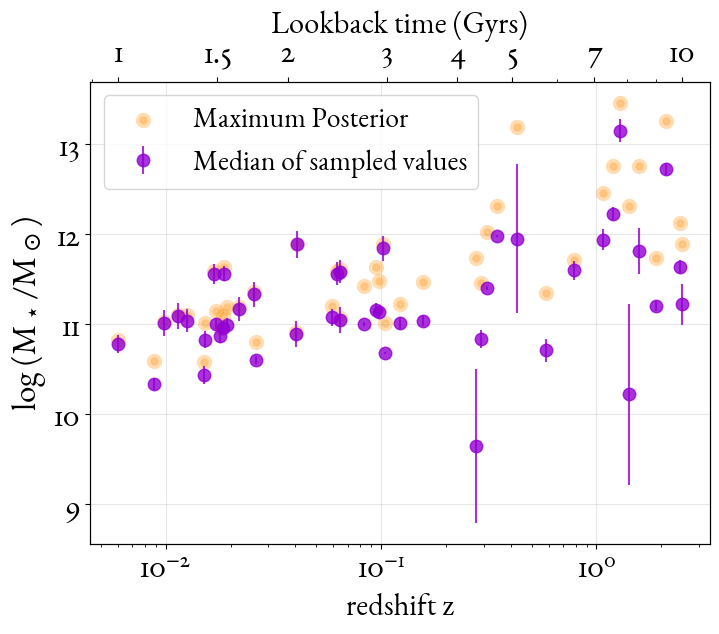
\includegraphics[width=\linewidth]{figures/ResultPlots/MassEvol_medianANDMaxPost.png}
    \caption{The 45 ARC Stellar Mass Evolution, stellar masses are calculated in Solar Mass units (M$_\odot$) and the base-ten logarithm of them is plotted. In bold color: the median of sampled values from the Bayesian process, uncertainties are half of the ($84^{\mbox{\tiny{th}}}$-$16^{\mbox{\tiny{th}}}$) percentile range. In light color: the maximum posterior value from the Bayesian process.}
    \label{fig:StarMassEvol}
\end{figure}
In Figure \ref{fig:StarMassEvol} the inferred stellar masses for each galaxy are plotted with the redshift (and lookback time). Assuming that the each galaxy is indicative of the ARC sample of massive, molecular gas-rich radiogalaxies, this can be interpreted as the evolution of ARC stellar content in the past $\sim 11$ Gyrs. \\
Both the median sampled value and maximum posterior value of total stellar mass are plotted for comparison of the sampling results, although the median value is used for science and the uncertainties are half of the ($84^{\mbox{\tiny{th}}}$-$16^{\mbox{\tiny{th}}}$) percentile range, as state-of-the-art practice\cite{Leja2020}. 
%----------------------------------------------------------------------------------%
%----------------------------------------------------------------------------------%
%----------------------------------------------------------------------------------%
\section{ARC Gas Mass to Stellar Mass Ratio } 
The molecular hydrogen (H$_2$) mass, probed by carbon monoxide (CO) gas emission all galaxies in the ARC survey has been calculated by Audibert et al. (2022)\cite{Audibert2022}. The gas mass-to-stellar mass ratio has been plotted in Figure \ref{fig:Gas-to-StarMassEvol} for the 45-ARC sample.

\label{sec:Res/ARC_MgasMstar}
\begin{figure}[htbp]
    \centering
    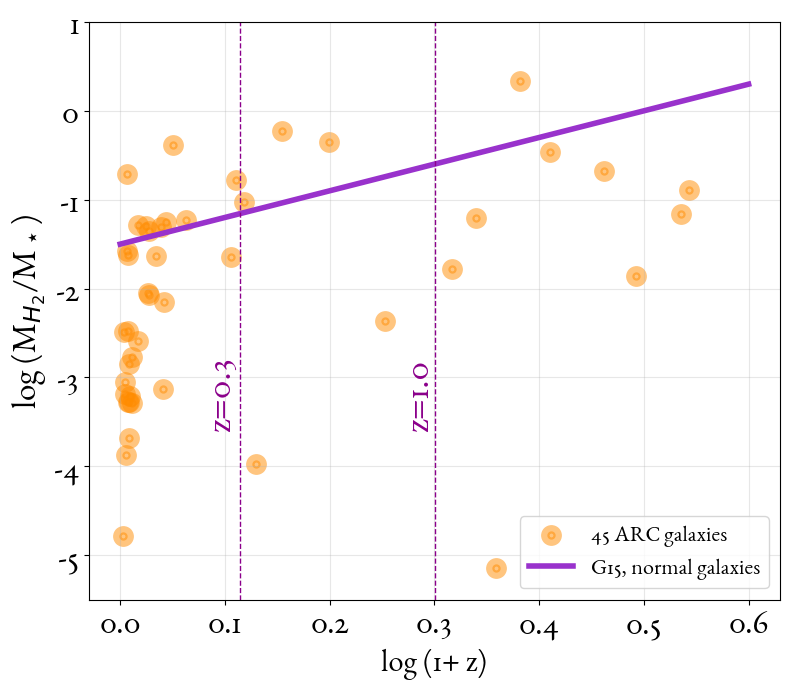
\includegraphics[width=0.64\linewidth]{figures/ResultPlots/GassToStars_median.png}
    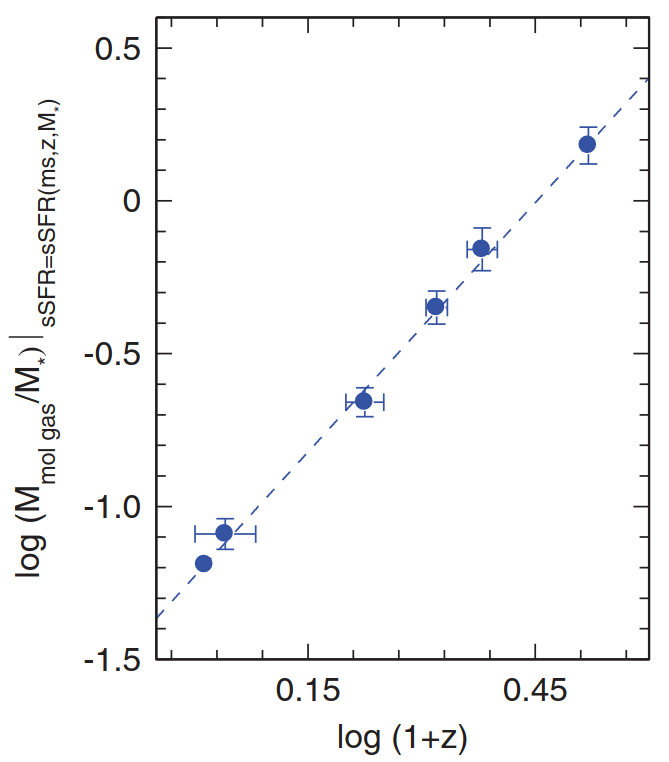
\includegraphics[width=0.35\linewidth]{figures/Genzel15.png}
    \caption{ The 45 ARC galaxies' gas-to-stellar mass ratio. Left panel: The Molecular hydrogen mass over the median total inferred stellar mass for each galaxy, the base-10 logarithm of the ratio is plotted with the base-10 logarithm of $(1+z)$, where $z$ is the redshift. The plotted line represents the main sequence and is adapted from Genzel et al. (2015)\cite{Genzel2015}. Right panel: The relation lifted from Genzel et al. (2015)\cite{Genzel2015} represents the main sequence galaxies.}
    \label{fig:Gas-to-StarMassEvol}
\end{figure}

%dependence of the CO-based molecular gas mass to stellar mass ratio at the main-sequence  \cite{Genzel2015}


%----------------------------------------------------------------------------------%
%----------------------------------------------------------------------------------%
%----------------------------------------------------------------------------------%
\section{ARC Stellar Mass Function} \label{sec:Res/ARC_SMF}
There are two main ways to estimate the stellar mass function for a galaxy sample\cite{Leja2020}, the first one is the $1/V_{\mbox{\tiny{max}}}$ method, introduced by Schmidt (1968)\cite{Schm1968} and refined by Avni \& Bahcall (1980)\cite{Avni1980} which calculates the number density of galaxies in bins of stellar mass with 
\begin{equation}
    \Phi_j = \dfrac{1}{\Delta \log M_{\star j}} \sum_{i=1}^N \, \dfrac{1}{V_{\mbox{\tiny{max}}}} \label{eq:SMF_schm} 
\end{equation} 
where $\Phi_j$ is the number density of galaxies in bin $j$, $\Delta \log M_{\star j}$ is the width in logarithmic scale of bin $j$, $N$ is the number of sources inside the bin and $V_{\mbox{\tiny{max}}}$ is the maximum comoving volume out to which these objects could be detected at the survey's limit. 
The second approach to estimate the stellar mass function is introduced by Sandage et al. (1979)\cite{Sand1979} and is a parametric maximum likelihood estimator that typically assumes the functional form of a Schechter\cite{Sche1976} function. 

%----------------------------------------------------------------------------------%
\subsection{Maximum Volume} \label{subsec:Res/V_max}
\subsubsection*{Calculating the Maximum Comoving Distance for a source}
As shown in equation \ref{eq:LumiD}: $ \;\; D_{\mbox{\tiny{L}}} = (1+z) \,D_{\mbox{\tiny{com}}} $\\
And from the definition of redshift: 
\begin{equation}
\nu_{\mbox{\tiny{obs}}} = \dfrac{\nu_{\mbox{\tiny{emitted, restframe}}}}{1+z_{\mbox{\tiny{source}}}}
\label{eq:redshift_freq}
\end{equation}
Virtually redshifting an isotropic source to $z_{\mbox{\tiny{limit}}}$, the observed photons at frequency $\nu_{\mbox{\tiny{limit}}} = 1.4\mbox{GHz}$ were emitted at frequency $\nu_{\mbox{\tiny{limit}}} = (1+z_{\mbox{\tiny{limit}}})\times1.4\mbox{GHz}$, the same holds for the observed redshift of the source, thus:
\begin{equation*} \begin{cases}
L_{\mbox{\tiny{bolom}}}\Big|_{\mbox{\tiny{observed}}}  = L_\nu \big( (1+z_{\mbox{\tiny{source}}})1.4\mbox{GHz} \big)\times (1+z_{\mbox{\tiny{source}}})1.4\mbox{GHz} \\ \\
L_{\mbox{\tiny{bolom}}}\Big|_{\mbox{\tiny{limit}}}  = L_\nu \big( (1+z_{\mbox{\tiny{limit}}})1.4\mbox{GHz} \big)\times (1+z_{\mbox{\tiny{limit}}})1.4\mbox{GHz}
\end{cases} \xRightarrow[]{\ref{eq:Flux-LumiD}}
\end{equation*}  
\begin{equation*} \xRightarrow[]{\ref{eq:Flux-LumiD}} \begin{cases}
L_{\mbox{\tiny{bolom}}}\Big|_{\mbox{\tiny{observed}}}  = f_{\mbox{\tiny{ν, obs}}}(1.4\mbox{GHz}) \times (1.4\mbox{GHz})  \times 4\pi \times D^2_{\mbox{\tiny{L}}} (z_{\mbox{\tiny{source}}} ) \\ \\
L_{\mbox{\tiny{bolom}}}\Big|_{\mbox{\tiny{limit}}} = f_{\mbox{\tiny{ν, limit}}}(1.4\mbox{GHz}) \times (1.4\mbox{GHz})  \times 4\pi \times D^2_{\mbox{\tiny{L}}} (z_{\mbox{\tiny{limit}}} )
\end{cases} 
\end{equation*} 
And since the bolometric luminosity of the source on its current redshift should be the same as its bolometric luminosity on the limit redshift (since there is no Doppler redshift from relativistic motion), the following is an identity:
\begin{equation*}
L_{\mbox{\tiny{bolom}}}\Big|_{\mbox{\tiny{observed}}}   = L_{\mbox{\tiny{bolom}}}\Big|_{\mbox{\tiny{limit}}} \xRightarrow[]{}  \end{equation*} 
\begin{equation*}
f_{\mbox{\tiny{ν, obs}}}(1.4\mbox{GHz}) \times D^2_{\mbox{\tiny{L}}} (z_{\mbox{\tiny{source}}} )  = f_{\mbox{\tiny{ν, limit}}}(1.4\mbox{GHz}) \times D^2_{\mbox{\tiny{L}}} (z_{\mbox{\tiny{limit}}} ) \xRightarrow[]{\ref{eq:LumiD}}  \end{equation*} 
\begin{equation} \xRightarrow[]{\ref{eq:Flux-LumiD}} (1+ z_{\mbox{\tiny{limit}}})^2 \times D^2_{\mbox{\tiny{com}}} (z_{\mbox{\tiny{limit}}} ) = \dfrac{f_{\mbox{\tiny{ν, obs}}}(1.4\mbox{GHz})}{f_{\mbox{\tiny{ν, limit}}}(1.4\mbox{GHz})} \times (1+ z_{\mbox{\tiny{source}}})^2 \times D^2_{\mbox{\tiny{com}}} (z_{\mbox{\tiny{source}}} )
\label{eq:Limit_f_D}
\end{equation}
In equation \ref{eq:Limit_f_D}, the right-hand-side is comprised entirely by known quantities:
\begin{itemize}
    \item $z_{\mbox{\tiny{source}}}$ is the spectroscopic redshift of each galaxy
    \item $f_{\mbox{\tiny{ν, obs}}}(1.4\mbox{GHz})$ is the observed flux at $1.4$GHz of each galaxy (bound to be greater or equal to $0.4$Jy, as a selection criterion of the ARC survey)
    \item $f_{\mbox{\tiny{ν, limit}}}(1.4\mbox{GHz}) $ is the limit flux at $1.4$GHz, which is equal to $0.4$Jy, for a galaxy to be marginally part of the ARC survey.\\
\end{itemize}
Solving the equation \ref{eq:Limit_f_D} for $\,z_{\mbox{\tiny{limit}}} $, it is trivial to calculate the limit comoving distance $ D_{\mbox{\tiny{com}}} (z_{\mbox{\tiny{limit}}} )$.
 
%---------------------------------------------------------------------------------%
\subsubsection*{Calculating the Maximum Volume for a source}
As discussed in section \ref{sec:Cosmo-ComovD}, the transverse comoving distance for a flat Universe is equal to the radial one $ D_{\mbox{\tiny{com, transv}}}  = D_{\mbox{\tiny{com}}}$.\\ 
The total volume of the solid angle layer spanned when virtually moving a galaxy from $z_{\mbox{\tiny{source}}}$ to $z_{\mbox{\tiny{limit}}}$ is 
\begin{equation}
\begin{aligned}
    V_{\mbox{\tiny{s}} \longrightarrow \mbox{\tiny{lim}}} &= V_{\mbox{\tiny{lim}}} - V_{\mbox{\tiny{s}}}=  \\ 
    & = \dfrac{4\pi}{3} \times \Big[ D^3_{\mbox{\tiny{com}}} (z_{\mbox{\tiny{limit}}} ) -  D^3_{\mbox{\tiny{com}}} (z_{\mbox{\tiny{source}}} )] 
\end{aligned} 
\label{eq:Volume_tot}
\end{equation}
The effective FOV of an ARC galaxy spans a solid angle $\Omega_{\mbox{\tiny{eff, ARC}}} = 75 \mbox{arcmin}^2 \approx 6.3462 \times 10^{-06}\; \mbox{steradian}$ (as discussed in Section \ref{sec:ARCsurv}), thus the maximum comoving volume spanned by the FOV of an ARC galaxy is
\begin{equation}
\begin{aligned}
    V_{\mbox{\tiny{max}}}  & = \dfrac{\Omega_{\mbox{\tiny{eff, ARC}}} }{4\pi}  \times \dfrac{4\pi}{3} \times \Big[ D^3_{\mbox{\tiny{com}}} (z_{\mbox{\tiny{limit}}} ) -  D^3_{\mbox{\tiny{com}}} (z_{\mbox{\tiny{source}}} )\Big] =\\
    & = \dfrac{\Omega_{\mbox{\tiny{eff, ARC}}} }{3} \times \Big[ D^3_{\mbox{\tiny{com}}} (z_{\mbox{\tiny{limit}}} ) -  D^3_{\mbox{\tiny{com}}} (z_{\mbox{\tiny{source}}} )\Big] =\\
    & = \dfrac{6.3462 \times 10^{-06}}{3} \times \Big[ D^3_{\mbox{\tiny{com}}} (z_{\mbox{\tiny{limit}}} ) -  D^3_{\mbox{\tiny{com}}} (z_{\mbox{\tiny{source}}} )\Big]
\end{aligned} 
\label{eq:Volume_max}
\end{equation}
%As discussed in Section \ref{sec:ARCsurv}, the ARC survey covers the sky north of $-40^o$ and south of  ($82\%$ of the celestial sphere)
%$\Omega_{\mbox{\tiny{eff, ARC}}} = 75 \mbox{arcmin}^2 \approx 6.3462 \times 10^{-06}\; \mbox{steradian}$
In Tables \ref{tab:ComplValues} and \ref{tab:ComplValues2}  the measured flux at 1.4 GHz (in units of Jansky) for each of the 45 sources is shown in the second column, the limit case redshift is shown on the fourth column for each source, the comoving volume through the FOV at the source in units of Mpc$^3$ is shown in the fifth column and the comoving volume through the FOV at the limit of each source in units of Mpc$^3$  is shown in the sixth column, according to the above calculations. 
%---------------------------------------------------------------------------------%
\subsection{Mass Completeness} \label{subsec:Res/MassCompl}
Estimating the Stellar Mass Function (which encompasses galaxy densities) is complicated by the presence of observational selection effects, for example due to detection thresholds. Statistical tools and techniques have been developed to identify, characterise and correct or remove the impact of observational selection effects from galaxy surveys.\\
Towards lower stellar masses, galaxies become intrinsically less luminous. This ultimately leads to a regime where the detection limits of the data are reached and galaxy number counts begin to fall as they are lost to noise.\\ %This study deduces that the ARC galaxies are on the massive end (\ref{fig:StarMassEvol}), nevertheless the mass completeness ought to be tested.\\  
The ARC galaxies are part of a flux limited survey, determining the completeness limit in stellar mass is not a trivial process, since there is not a sharp limit in stellar mass corresponding to the sharp limit in flux\cite{Marches2009}. Here the approach of Weigel et al. (2016)\cite{Weigel2016} is followed, where $M_{\star, \mbox{\tiny{limit}}}$ of each galaxy is Mass-to-Light ratio ($M/L$) dependent. The ($M/L$) of each galaxy is considered constant, consequently proportional to the mass-to-flux ratio for fixed redshift, thus the $M_{\star, \mbox{\tiny{limit}}}$ can be defined
\begin{equation*}
    \dfrac{M_{\star,\mbox{\tiny{source}}}}{L_{1.4\mbox{\tiny{GHz, source}}}(z_{\mbox{\tiny{source}}})}  \propto \dfrac{M_{\star,\mbox{\tiny{source}}}}{f_{1.4\mbox{\tiny{GHz, source}}} (z_{\mbox{\tiny{source}}}) }  = \dfrac{M_{\star,\mbox{\tiny{limit}}}}{f_{1.4\mbox{\tiny{GHz,limit}}} (z_{\mbox{\tiny{source}}}) } \iff
\end{equation*}
\begin{equation}
    \iff M_{\star, \mbox{\tiny{limit}}} = \dfrac{f_{1.4\mbox{\tiny{GHz,limit}}} (z_{\mbox{\tiny{source}}})}{f_{1.4\mbox{\tiny{GHz, source}}} (z_{\mbox{\tiny{source}}})} \times M_{\star,\mbox{\tiny{source}}} \label{eq:MassCompl}
\end{equation}
The base-ten logarithm of stellar mass in units of solar masses is shown in the seventh column of Tables \ref{tab:ComplValues} and \ref{tab:ComplValues2}, as well as the mass limit in the last column, also in base-ten logarithm of stellar mass in units of solar masses.
Calculating the stellar mass completeness limit for each galaxy individually, it is ascertained that the working sample of 45 sources is stellar mass complete, as shown in Figure \ref{fig:MassCompl}.
%and thus has to be determined for each source individually.
%for a flux-limited sample is particularly challenging, since there is not a sharp limit in stellar mass corresponding to the sharp limit in flux
%completeness in stellar mass based on the maximal stellar mass allowed for a galaxy at the flux limit of the sample. This maximal mass is typically taken to be the stellar mass of a passively evolving population with no dust extinction formed in a single burst at very high (z ∼ 10) redshift, scaled to match the limiting flux (SSP-derived completeness limit, hereafter).
\begin{figure}[htbp]
    \centering
    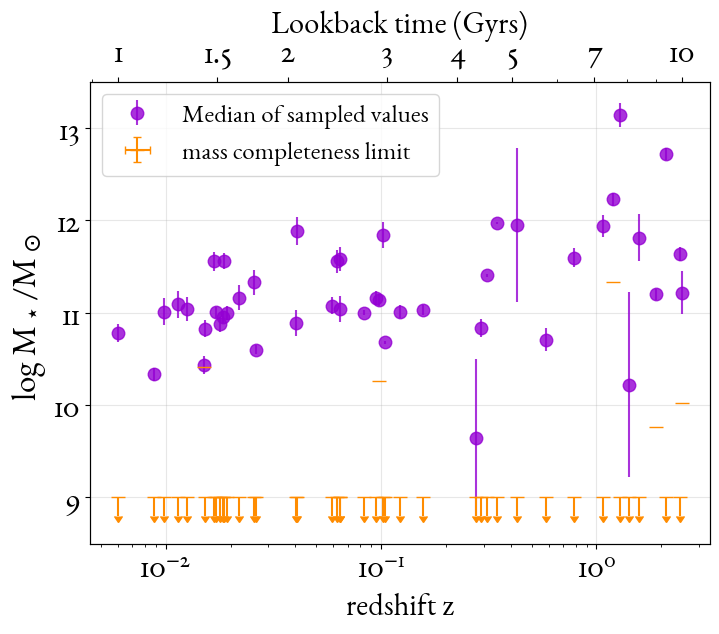
\includegraphics[width=\linewidth]{figures/ResultPlots/Mass_Compl.png}
    \caption{The mass completeness limits for each, derived for each galaxy assuming a constant M/L ratio and consequently a constant stellar mass-to-flux ratio. For 40 out of 45 total galaxies the limit $\log M_{\star, \mbox{\tiny{limit}}}$ is lower than 9, in which case it is shown at the $9$-level with an upper limit arrow. The working sample is $100\%$ mass complete.}
    \label{fig:MassCompl}
\end{figure}

%---------------------------------------------------------------------------------%
\subsection{NVSS Completeness Correction} \label{subsec:Res/ComplCorr}
\begin{figure}
    \centering
    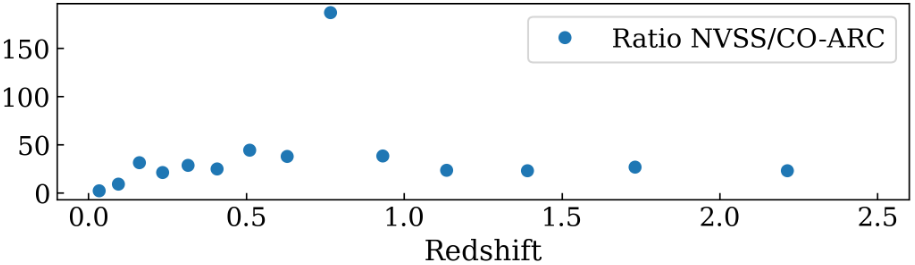
\includegraphics[width=.7\linewidth]{figures/AudibertCompleteness.png}
    \caption{The NVSS completeness correction so that by multiplying the final ARC source sample in different redshift intervals can reproduce the number of sources in the NVSS survey. Plot lifted from Audibert et al. (2022)\cite{Audibert2022} for the complete ARC survey.}
    \label{fig:ComplPlot}
\end{figure}
In order to estimate the stellar mass function the $1/V_{\mbox{\tiny{max}}}$ method is adopted here, and for the purposes of the ARC survey (which is representative of the NVSS survey) the equation \ref{eq:SMF_schm} is modified to 
\begin{equation}
\Phi_j = \dfrac{1}{\Delta \log M_{\star j}} \sum_{i=1}^N \, \dfrac{\omega(\delta z) }{V_{\mbox{\tiny{max}}}} \label{eq:SMF_arc}
\end{equation}
where $\omega (\delta z)$ is a weight corresponding to the completeness correction with respect to the NVSS survey , that is:
%addopted by Audibert et al. (2022)\cite{Audibert2022} and shown in Figure \ref{fig:ComplPlot}, that is 
\begin{equation}
\omega(\delta z) = \dfrac{\mbox{\small{Number of NVSS sources with spectroz in δz slice per sterad}}}{\mbox{\small{Number of ARC sources with spectroz in δz slice per sterad}}}=  \dfrac{\dfrac{N_{\mbox{\tiny{NVSS}}}(\delta z)}{\Omega_{\mbox{\tiny{NVSS}}}}} { \dfrac{N_{\mbox{\tiny{ARC}}}(\delta z)}{\Omega_{\mbox{\tiny{eff, ARC}}}} } 
\label{eq:weights_arc}
\end{equation}
where $\Omega_{\mbox{\tiny{eff, ARC}}}$ is the ARC survey's effective field of view (as discussed in Section \ref{sec:ARCsurv}), $\Omega_{\mbox{\tiny{NVSS}}}$ is the NVSS survey's coverage of the celestial sphere, $N_{\mbox{\tiny{ARC}}}(\delta z)$ is the total number of ARC sources in a redshift region  $\delta z$ and $N_{\mbox{\tiny{NVSS}}}(\delta z)$ is the number of NVSS sources with spectroscopically confirmed redshift in the same redshift region.\\ %where $\Omega_{\mbox{\tiny{tot, ARC}}}$ is the ARC survey's coverage of the celestial sphere's solid angle, $\Omega_{\mbox{\tiny{tot, NVSS}}}$ is the NVSS survey's coverage of the celestial sphere, $N_{\mbox{\tiny{ARC}}}(\delta z)$ is the total number of ARC sources in a redshift region  $\delta z$ and $N_{\mbox{\tiny{NVSS}}}(\delta z)$ is the number of NVSS sources with spectroscopically confirmed redshift in the same redshift region.\\ %As shown in equation \ref{eq:OmegaTotARC}, the ARC survey covers a solid angle of $\Omega_{\mbox{\tiny{tot, ARC}}} = 3.94\pi \;\mbox{steradian}$
The NVSS survey\cite{NVSS} covers the sky north of $-40^o$, that is 
\begin{equation*}
    \Omega_{\mbox{\tiny{tot, NVSS}}} = \int_{0}^{2\pi}\,d\phi\, \int_{-2\pi/9}^{\pi}\, \cos \theta\,d\theta = 2\pi \times (1+\sin\frac{2\pi}{9}) \; \mbox{steradian}= 3.28 \pi\; \mbox{steradian}
\end{equation*}
Audibert et al. (2022)\cite{Audibert2022} calculate the total number of NVSS sources within the redshift interval $z\in[0,2.5]$ (which is the redshift range of the entire ARC sample) to be $N_{\mbox{\tiny{NVSS, tot}}} =  9331$ and in order to estimate the number of NVSS sources with spectroscopic redshift, a fraction of $f_{\mbox{\tiny{spectro z}}} = 0.06$ is assumed based on other surveys (SDSS and FIRST), leading to $N_{\mbox{\tiny{NVSS}}} = 0.06\times 9331 = 559.86$.\\
Although the total number of ARC sources with spectroscopic redshift is 120, the present work used 45 for science, thus the NVSS completeness correction for the redshift range of $z\in[0,2.5]$ is (based in equation \ref{eq:weights_arc}):
\begin{equation}\begin{aligned}
    \omega(0< z<2.5) &= \dfrac{N_{\mbox{\tiny{NVSS}}}(0< z<2.5)}{\Omega_{\mbox{\tiny{NVSS}}}} \times  \dfrac{\Omega_{\mbox{\tiny{eff,ARC}}}}{N_{\mbox{\tiny{ARC}}}(0< z<2.5)}  =  \\ 
    & = \dfrac{559.86}{3.28 \pi \;\mbox{sterad}} \times  \dfrac{6.346\times10^{-6} \;\mbox{sterad}}{45} = \\ & = 7.66\times10^{-6}
    \end{aligned} 
\label{eq:weight_tot}
\end{equation}
Since the ratio of sources $N_{\mbox{\tiny{NVSS}}}(0< z<2.5)/N_{\mbox{\tiny{CO-ARC}}}(0< z<2.5)$ in the work of Audibert et al. (2022)\cite{Audibert2022} is roughly similar for the sub-sample of 66 ARC galaxies in different redshift bins (as shown in Figure \ref{fig:ComplPlot}), a constant weight for NVSS correction is adopted here (equation \ref{eq:weight_tot}). All relevant values for the completeness limit calculation of each galaxy are shown in Table \ref{tab:ComplValues} and \ref{tab:ComplValues2}

%--------------------------------------------------------------------------------------------
\subsection{Redshift Ranges} \label{subsec:Res/Redbins}

Following the regime of Audibert et al. (2022)\cite{Audibert2022} the 45 ARC sample is divided in three redshift ranges of $0.006<z<0.3$, $0.3<z<1.0$ and $1.0<z<2.5$, respectively. 31 out of 45 galaxies fall into the first redshift range ($0.006<z<0.3$), and are dividend in three mass bins of mean Stellar Mass in base-ten logarithmic scale of 10.516, 11.006 and 11.554 containing 8, 12 and 11 galaxies respectively. 31 out of 45 galaxies fall into the first redshift range ( $0.006<z<0.3$), and are dividend in three mass bins of mean Stellar Mass : $10^{10.516}\;\mbox{M}_\odot$, $10^{11.006}\;\mbox{M}_\odot$ and $10^{11.554}\; \mbox{M}_\odot$ containing 8, 12 and 11 galaxies respectively.
The redshift ranges of $0.3<z<1.0$ and $1.0<z<2.5$ gather 5 and 9 galaxies respectively. For the $0.3<z<1.0$ redshift range the mean Stellar Mass is $10^{11.525}\;\mbox{M}_\odot$ and for $1.0<z<2.5$ redshift range the mean Stellar Mass is $10^{11.788}\;\mbox{M}_\odot$. The following table shows all relevant values used for constructing the Stellar Mass Function, while the Stellar Mass Function is plotted and shown in Figure \ref{fig:ARC_SMF}\\
%\begin{table}    \caption{Crucial values and limits for calculating completeness of 45 ARC galaxies} \label{tab:ARC_45redbins} 3.34005038e-03 1.43659043e-04 6.71958271e-05
\begin{tabular}{cccccc}
    \addlinespace
    \hline  %\toprule
    {} & Redshift range & N &  Mean [$\log M_\star/M_\odot$] &   $\Delta \log M_\star$ & $\Phi$  \\
    \hline   %\midrule
    \hline   %\midrule
    %---------------------------------------------% 
    %-----  0  ---------%
    bin 1 & $0<z<0.3$ & 8 & 10.516  & 1.1843  & $3.34\times10^{-3}$ \\      
    %-----  1  ---------%    
    bin 2  & $0<z<0.3$ & 12 & 11.006  & 0.2028  &  $1.44 \times10^{-4}$ \\
    %-----  2  ---------% 
    bin 3 & $0<z<0.3$ & 11 & 11.554  & 0.7928   & $6.72 \times10^{-5}$\\
    \hline
    %-----  3  ---------%
    binned all  & $0.3<z<1.0$ & 5 & 11.525 & 1.2642   & $2.71 \times10^{-9}$\\
    \hline
     %-----  5  ---------%
    binned all & $1.0<z<2.5$ & 9  & 11.788  & 2.9204   & $6.31 \times10^{-10}$\\
    \hline
    \end{tabular} \\ \\
%\end{table}
Where N is the number of galaxies in each bin, and $\Phi$ is the quantity $$\Phi = \dfrac{1}{\Delta \log M_{\star }} \sum_{i=1}^N \, \dfrac{\omega(\delta z) }{V_{\mbox{\tiny{max}}}}$$ for each bin. In the final plot (Figure \ref{fig:ARC_SMF}) each bin is represented by one point, the color distinguishes the redshift ranges and the point size is proportional to the number of galaxies in each bin.


\begin{xltabular}{\textwidth}{cccccccc}
    \caption{Values and limits for calculating completeness of 45 ARC galaxies. The name of each source is shown in the first column, in the second column is the 1.4 GHz flux in units of Jansky, the redshift of the source and the limit case redshift are in the third and fourth column respectively, the comoving volume through the FOV at the source and at the limit case are shown in the fifth and sixth column. The median sampled base-ten logarithm of stellar mass in units of solar masses and the limit case stellar mass (in the same regime) are in seventh and eighth columns, respectively. } \label{tab:ComplValues}\\
    \toprule
    Source name & $f_{\mbox{\tiny{1.4GHz, source}}}$ &  $z_{\mbox{\tiny{source}}}$ & $z_{\mbox{\tiny{limit}}}$  & V$_{\mbox{\tiny{com, source}}}$ & V$_{\mbox{\tiny{com, limit}}}$ & logM$_{\star, \mbox{\tiny{source}}}$ & logM$_{\star, \mbox{\tiny{limit}}}$  \\
    \midrule
    \midrule
    \endfirsthead
        \caption{Values and limits for calculating completeness of 45 ARC galaxies - continued} \label{tab:ComplValues2}\\
    \toprule
    %\toprule
    Source name & $f_{\mbox{\tiny{1.4GHz, source}}}$ &  $z_{\mbox{\tiny{source}}}$ & $z_{\mbox{\tiny{limit}}}$  & V$_{\mbox{\tiny{com, source}}}$ & V$_{\mbox{\tiny{com, limit}}}$ & logM$_{\star, \mbox{\tiny{source}}}$ & logM$_{\star, \mbox{\tiny{limit}}}$  \\
    \midrule
    \midrule
    \endhead
    %-----  0  ---------%
    J0006-0623 & 1.754 & 0.347 & 0.644  & 10621412470 & 53619010921  & 11.973 & 2.731  \\*      
    %-----  1  ---------%    
    J0009-3216  & 0.505 & 0.026 & 0.029  & 5451077 & 7667186  & 11.329 & 8.970  \\*
    %-----  2  ---------% 
    J0048+3157 & 0.401 & 0.015 & 0.015  & 1106755 & 1110842  & 10.434 & 10.408 \\*
    %-----  3  ---------%
    J0057+3021 & 1.715 & 0.017 & 0.034  & 1518505 & 12811912  & 11.554 & 2.694 \\*
     %-----  5  ---------%
    J0106-4034 & 0.801 & 0.584 & 0.776  & 42025675299 & 84426729631  & 10.708 & 5.349\\*
     %-----  6  ---------%
    J0112-6634 & 0.431 & 1.189 & 1.226  & 218963612672 & 233195025541  & 12.224 & 11.333 \\*
     %-----  8   ---------%
     J0119+3210 & 2.502 & 0.059 & 0.140  & 65948906 & 826594905  & 11.074 & 1.771 \\*
     %-----  9  ---------%
     J0125-0005  & 1.467 & 1.076 & 1.821  & 177158540511 & 495526195715  & 11.933 & 3.255  \\*
     %-----  16 (cont 2)  ---------%
     J0327-2239  & 0.459 & 1.898 & 2.007  & 532781704065 & 585503176478  & 11.196 & 9.759 \\*
     %-----  19  ---------%
     J0504-1014 & 1.461 & 0.040 & 0.075  & 21020608 & 132875955  & 10.890 & 2.982\\*
     %-----  25  ---------%
     J0758+3747& 1.734 & 0.041 & 0.083  & 21772604 & 174619443  & 11.883 & 2.742 \\*
     %-----  28  ---------%
     J0840+2949 & 0.514 & 0.065 & 0.073  & 85292621 & 121422757  & 11.041 & 8.591 \\*
     %-----  30  ---------%
      J0914+0245 & 0.576 & 0.427 & 0.497  & 18591860833 & 27803371016  & 11.947 & 8.295  \\*
     %-----  35  ---------%
      J1000-3139 & 0.534 & 0.009 & 0.010  & 222904 & 342648  & 10.333 & 7.737 \\*
     %-----  36  ---------%
      J1008+0029 & 0.434 & 0.098 & 0.102  & 286702369 & 320847780  & 11.135 & 10.259 \\*
     %-----  51  ---------%
      J1248-4118 & 3.922 & 0.010 & 0.030  & 313986 & 9075331  & 11.011 & 1.123  \\*
     %-----  52  ---------%
      J1301-3226 & 1.227 & 0.017 & 0.030  & 1609884 & 8337450  & 11.001 & 3.586 \\*
     %-----  55  ---------%
      J1336-3357 & 4.372 & 0.013 & 0.040  & 637246 & 21216550  & 11.037 & 1.010  \\*
     %-----  56  ---------%
      J1348+2635 & 0.700 & 0.064 & 0.084  & 84285576 & 184699036  & 11.580 & 6.617  \\*
     %-----  60  ---------%
      J1407-2701 & 0.708 & 0.022 & 0.029  & 3357927 & 7742971  & 11.163 & 6.308 \\*
     %-----  67  ---------%
      J1602+0157 & 8.286 & 0.105 & 0.405  & 352065728 & 16146030943  & 10.678 & 0.515  \\*
     %-----  72  ---------% 
     J1945-5520 & 0.679 & 0.015 & 0.020  & 1132482 & 2470867  & 10.827 & 6.379  \\*
     %-----  77  ---------% 
      J2131-3837 & 0.764 & 0.018 & 0.025  & 2057386 & 5319099  & 10.951 & 5.735  \\*
     %-----  79  BREAK HERE!---------% 
      J2134-0153 & 1.880 & 1.285 & 2.413  & 256903577664 & 785233255541  & 13.141 & 2.796 \\*
    %-----  82  ---------% 
     J2257-3627 & 0.840 & 0.006 & 0.009  & 71176 & 214877  & 10.781 & 5.134  \\*
    %-----  83  ---------% 
     J2320+0812 & 0.627 & 0.011 & 0.014  & 478432 & 930838  & 11.090 & 7.076  \\ \addlinespace
    %-----  85  ---------% 
     J2325-1207 & 1.627 & 0.083 & 0.159  & 177577734 & 1187583652  & 11.000 & 2.705  \\*
    %-----  86  ---------% 
     J2341+0018 & 0.473 & 0.277 & 0.298  & 5698161687 & 6983071317  & 9.647 & 8.153  \\*
    %-----  93  ---------%
      J0125-0122 & 0.826 & 0.018 & 0.026  & 1879930 & 5456446  & 10.871 & 5.263 \\*
    %-----  94  ---------%
    J0156+0537 & 0.635 & 0.019 & 0.024  & 2138230 & 4217506  & 11.555 & 7.279   \\*
    %-----  95  ---------%
    J0709+4836 & 0.512 & 0.019 & 0.022  & 2329418 & 3345999  & 10.993 & 8.593\\*
    %-----  96  ---------%
    J2214+1350 & 2.216 & 0.026 & 0.060  & 5780173 & 68352752  & 10.598 & 1.913  \\*
    %-----  103  ---------%
    J1348+2635 & 0.925 & 0.063 & 0.093  & 77671998 & 250804892  & 11.558 & 4.998 \\*
    %-----  105  ---------%
     J1321+4235 & 1.687 & 0.790 & 1.415  & 88089040027 & 310812208203  & 11.593 & 2.748 \\*
    %-----  108  ---------%
    J1531+2404 & 3.352 & 0.095 & 0.250  & 262964983 & 4287716737  & 11.160 & 1.332  \\*
    %-----  109  ---------%
    J0747-1917 & 2.003 & 0.102 & 0.213  & 326279961 & 2739578035  & 11.841 & 2.365 \\*
    %-----  111  ---------%
    J0009+1244 & 1.528 & 0.156 & 0.283  & 1118836863 & 6099733607  & 11.028 & 2.888  \\*
    %-----  112  ---------%
    J011651-2052 & 3.723 & 1.410 & 3.524  & 308966929051 & 1325168544618  & 10.221 & 1.098  \\*
    %-----  113  ---------%
    J0234+3134 & 0.909 & 1.575 & 2.201  & 381597436448 & 680202950647  & 11.811 & 5.199  \\*
    %-----  114  ---------%
    J0408-2418 & 0.629 & 2.433 & 2.934  & 795973831784 & 1042737809694  & 11.636 & 7.398  \\*
    %-----  115  ---------%
    J2106-2405 & 0.447 & 2.491 & 2.609  & 824465074464 & 882462629500  & 11.217 & 10.026 \\*
    %-----  116  ---------%
    J0242-2132 & 1.013 & 0.312 & 0.463  & 7954274949 & 23099299235  & 11.402 & 4.504  \\*
    %-----  117  ---------%
    J1305-1033 & 0.843 & 0.291 & 0.401  & 6551933406 & 15702640284  & 10.832 & 5.138  \\*
    %-----  118  ---------%
    J0403+2600 & 1.285 & 2.109 & 3.417  & 635471606586 & 1274807911997  & 12.714 & 3.958  \\*
    %-----  119  ---------%
    J1347+1217 & 5.375 & 0.122 & 0.387  & 548578299 & 14305603664  & 11.011 & 0.819  \\*
\end{xltabular}



\begin{figure}
    \centering
    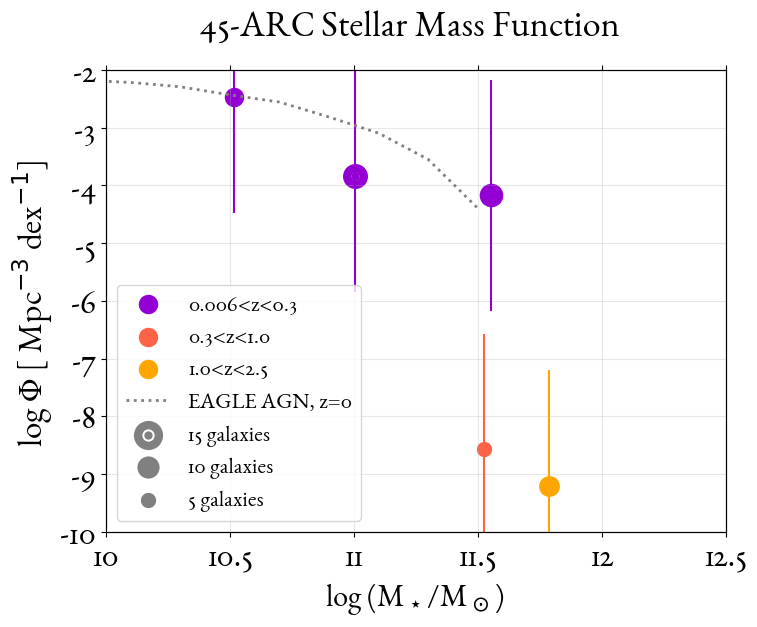
\includegraphics[width=\linewidth]{figures/ResultPlots/SMF_compl_werr.png}
    \caption{The galaxy Stellar Mass Function with and its evolution in three redshift ranges. The color distinguishes the redshift ranges and the point size is proportional to the number of galaxies in each bin. The SMF for AGNs of the EAGLE\cite{EAGLE} simulation at redshift $z=0$ is plotted for comparison.}
    \label{fig:ARC_SMF}
\end{figure}






%$\Omega_{\mbox{\tiny{tot, NVSS}}} = 0.82 \times 4\pi\; \mbox{steradian} = 3.28 \pi\; \mbox{steradian}$ 
%Audibert et al. (2022)\cite{Audibert2022} calculate the parametres for completeness correction in the redshift interval $z\in[0,2.5]$ that covers the entire ARC sample, given that the effective FOV of the ARC survey is $\Omega_{\mbox{\tiny{eff, ARC}}} = 75 \mbox{arcmin}^2 \approx 6.3462 \times 10^{-06}\; \mbox{steradian}$,  the FOV of the NVSS survey is $\Omega_{\mbox{\tiny{eff, NVSS}}} = 3.27 \pi\; \mbox{steradian}$, $N_{\mbox{\tiny{NVSS, tot}}} =  9331$ is the total number of NVSS sources with $z\in[0,2.5]$ and in order to calculate the number of NVSS sources with spectroscopic redshift, a fraction of $f_{\mbox{\tiny{spectro z}}} = 0.06$ is assumed based on other surveys (SDSS and FIRST), leading to $N_{\mbox{\tiny{NVSS}}} = 0.06\times 9331 = 559.86$ and the correction for $z\in[0,2.5]$ :
%$$ \omega_i = \dfrac{559.86}{3.27 \pi} \times \dfrac{6.3462 \times 10^{-06}}{ N_{\mbox{\tiny{ARC}}}(z\in[0,2.5])} $$








%\subsection{Exemplary Figure Referencing}\label{subsec:Section_Name/fig_rfs}
%See Figure \ref{fig:UoC} for details. Additional information can befound in the footnote \footnote{Image taken from \url{https://en.wikipedia.org/wiki/File:Siegel_Uni-Koeln_(Grau).svg}.}.


















